\chapter{Compilers and analysis tools}

\change[inline]{TODO: Add more tools.}

In the previous chapter, the reader was introduced to a branch of program
ana\-ly\-sis. 
The techniques discussed above focused on both the static and runtime
side of program analysis. 

Regardless of whether these approaches have been implemented, it was 
required to find a suitable tool for source code manipulation for two reasons. 
First, any external tool output might require altering the input source code 
based on its output. 
Second, if implementing any code reducing algorithm would have to occur, 
one would need a sophisticated code modifying framework. 

Due to these reasons, an analysis of compilers and tools for C and C++ was conducted. 
The goal of the analysis is to pick the most practical tool available. 
Required criteria include frequent upkeep of the framework, 
an existing user base, and the ability to manipulate some abstract 
representation of the code.

The representation boiled down to an abstract syntax tree (AST). 
AST embodies the syntactic structure of the code, regardless of the code's language. 
A vertex of an AST represents a construct of the code while not being concrete 
with the programming language's details. 
This generality is perfect for C and C++'s chosen domain, 
as both languages only differ syntax-wise in minor details.

\change[inline]{TODO: Add more text about AST.}

Below are the findings concerning the most important candidates.

\section{GCC}

A well known C and C++ compiler, the GNU Compiler Collection is an extensive
open source project. 
As popular as GCC is, it does not provide the features an analysis-tool-building 
developer needs. 

For the sake of building such tools, a compiler front end is used. 
Due to an old design, it is difficult to work with either the front end or 
the back end of GCC alone. 
Besides, the compiler implicitly makes optimizations that destroy any parallels 
between the source code and the AST. 
Therefore, the AST has to be treated as an entirely different object rather than 
an abstraction of the code. 
Most of the compiler's source code representation is unintuitive and 
hard to pick up for anyone not actively contributing to GCC. 
Figure~\ref{img:gcc} showcases the unfriendliness rather well.
Compared to figure~\ref{img:pdg}, which is an output of a tool built using
LLVM and Clang, GCC's mapping between the source code and the internal
representation does not hold up.

As far as AST manipulation is concerned, the compiler allows the user to dump 
the structure into a text representation. 
However, due to the difficulties mentioned above, it can hardly be used.

\begin{figure}[p]\centering
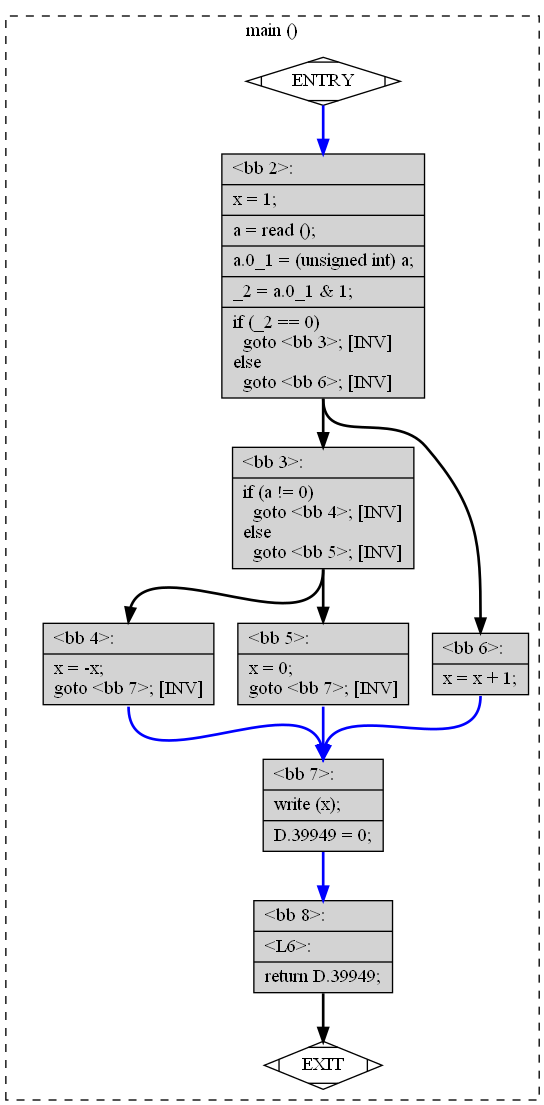
\includegraphics[scale=0.55]{gcc_ast}
\caption{GCC AST Dump. This figure showcases 
the AST representation of~\ref{lst:simpleexample}
as dumped by GCC. Note that it is not easily comprehendable.}
\label{img:gcc}
\end{figure}

These issues result in a seldom-used variant that offers nearly 
no developer-friendly features. 
An upside is that GCC allows the user to visualize the AST. 
However, that is hardly a useful feature in the context of this paper.

\section{Clang}

Thanks to LLVM, the widespread compiler infrastructure, the Clang project 
has provided a compiler front end not only for C and C++ but also 
for CUDA, OpenCL, and other languages. 
The extend of Clang as a compiler front end is so vast that it covers 
both the C++ standard and the unofficial GNU++ dialect.

The project does not include just the front end but also a static analyzer 
and several code analysis tools, which are now commonly used in IDE's as 
syntax and semantic checks. 

This description of Clang foreshadows its friendliness to analysis tool developers. 
The fact that the front end runs on a common intermediate language also indicates 
that openly working with abstract code representations is supported.

\change[inline]{TODO: Add more general text based on what I write in the Clang chapter.}

\section{Summary}

While the chapter only highlighted two significant candidates, the analysis 
looked at a plethora of tools. 
Those, however, were not able to compete feature-wise due to the sheer size 
and extent of GCC and Clang. 

It would seem that parsing multiple programming languages into an abstract 
representation requires a common intermediate language, in which 
the representation is stored. 
Having an intermediate language is not always possible for several reasons, 
including licensing and old architecture. 
The compiler giant GCC seems to suffer from precisely that.
Additionally, since the Clang project is being contributed to regularly, 
resulting in as many as five releases per year, 
it pulls in a more significant developer community. 

Therefore, Clang is the favorite source code altering tool for this project. 
In the following chapter, the relevant parts of the Clang project 
will be broken down and explained.